%
% 0_einleitung.tex -- Einleitung
%
% (c) 2020 Prof Dr Andreas Müller, Hochschule Rapperswil
%
% !TEX root = ../../buch.tex
% !TEX encoding = UTF-8
%

Das Weltall hat uns Menschen und Mathematiker schon immer fasziniert und inspiriert. 
Seit Mitte des 20. Jahrhunderts ist es möglich, Raketen in den Weltraum zu schicken. 
Die Berechnung der Flugbahn von der Erde in eine Umlaufbahn stellt dabei ein klassisches Variationsproblem dar. 
\index{Umlaufbahn}%
Ziel ist es, die optimale Flugbahn zu finden, die den Treibstoffverbrauch minimiert und dabei alle relevanten Einflüsse berücksichtigt.
\index{Treibstoffverbrauch}%

In der Regelungstechnik gibt es viele solcher Variationsprobleme,
\index{Regelungstechnik}%
doch die Komplexität einer Raketenflugbahn ist besonders herausfordernd.
Diese hängt von zahlreichen Faktoren ab, wie der Massenänderung der
Rakete, dem Einfluss der Atmosphäre sowie den aerodynamischen
\index{Rakete}%
\index{Atmosphäre}%
\index{Massenänderung}%
Kräften.
Insbesondere die Steuerung der Rakete, um die Verluste durch
Schwerkraft und Luftwiderstand zu minimieren, spielt dabei eine
\index{Verlust}%
zentrale Rolle.

Dieses Kapitel zeigt, wie man ein so komplexes Problem vereinfachen
kann, um eine realitätsnahe Lösung zu erhalten.
Es werden die grundlegenden Bewegungsgleichungen, Randbedingungen,
sowie die Techniken der Variationsrechnung vorgestellt, um die
optimale Flugbahn zu berechnen.
Dabei wird auch das Pitchover-Manöver näher untersucht, das
\index{Pitchover}%
entscheidend zur Reduktion der Energieverluste beiträgt.

\begin{figure}
\centering
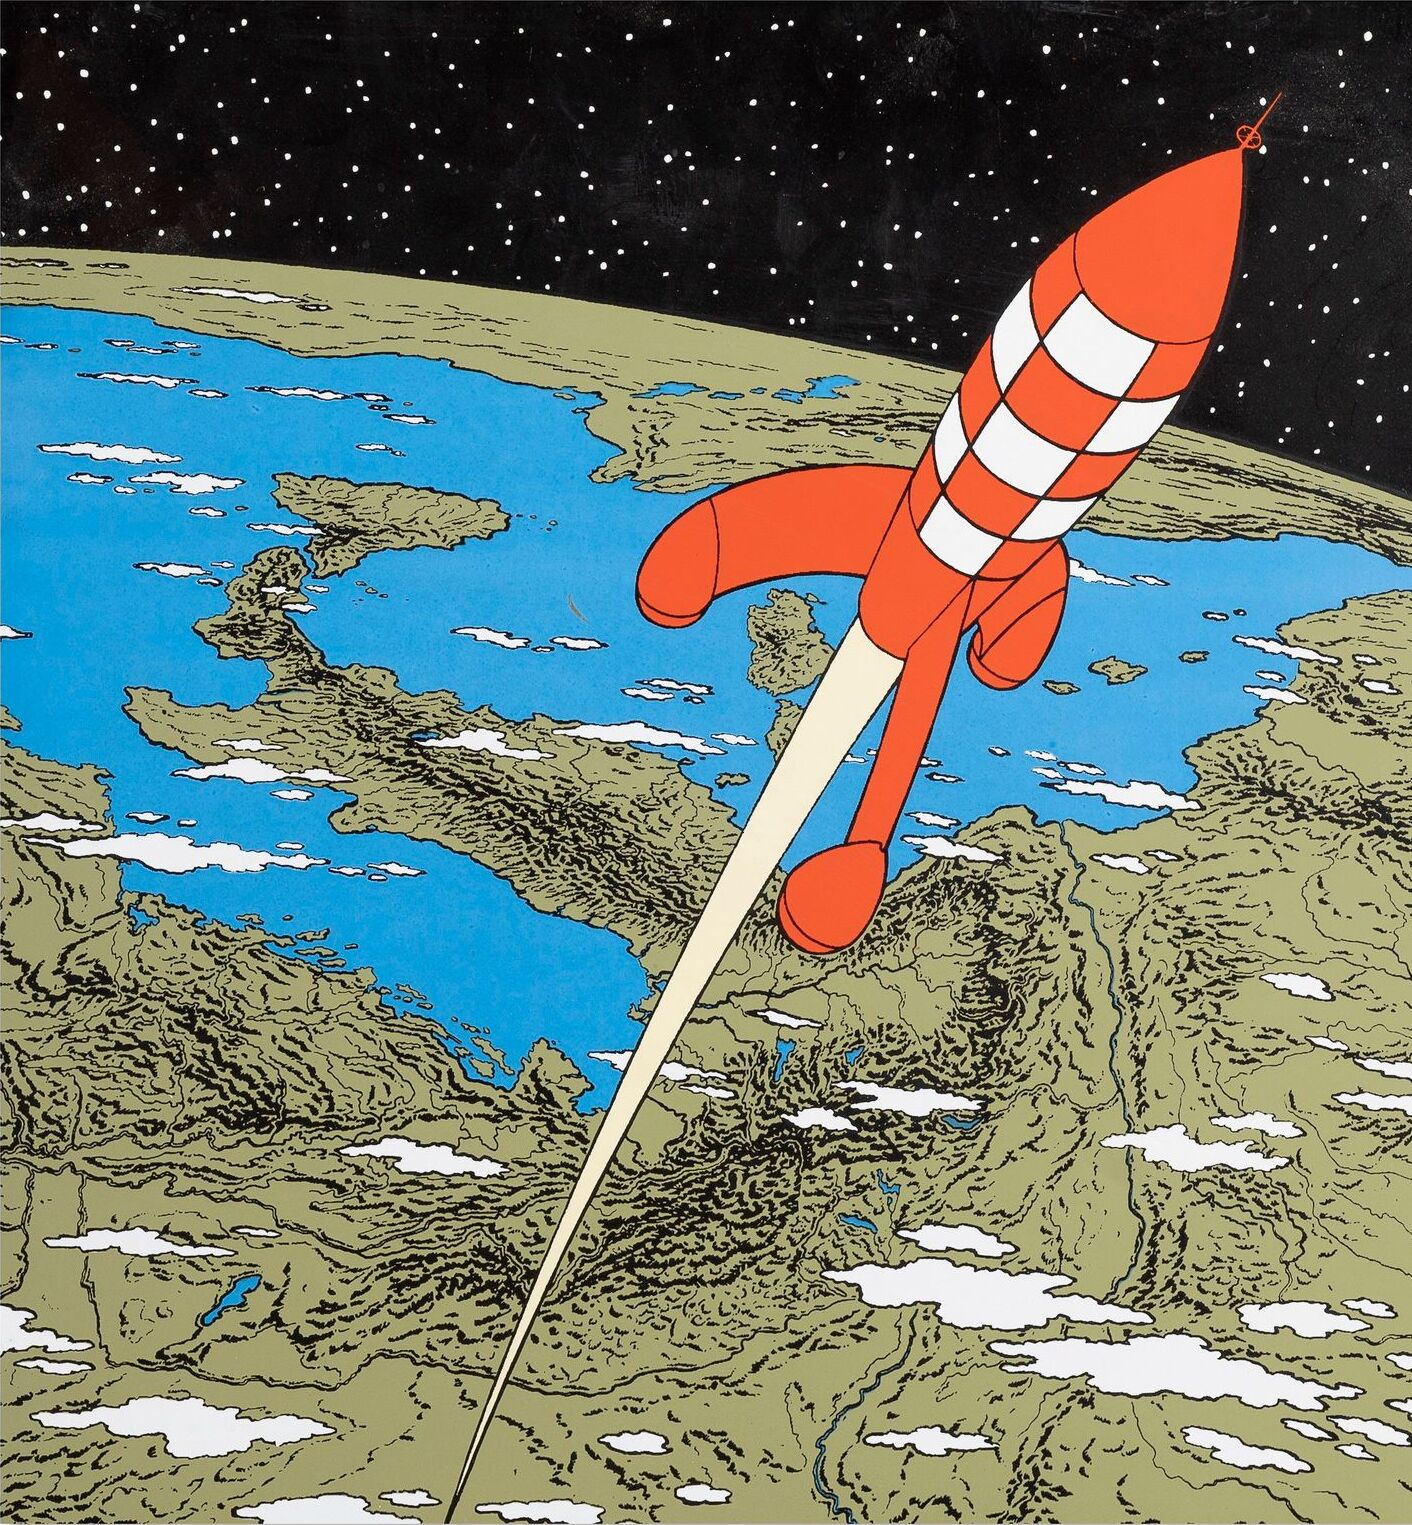
\includegraphics[width=1.0\linewidth]{papers/leo/Grafiken/raketen_typen-cropped.jpg}
\caption{Als 1953 der Tim und Struppi-Band {\em Reiseziel Mond}
erschien, war dies für viele Menschen noch schwer vorstellbar
\cite{leo:timstruppi}.
\index{Tim und Struppi}%
}
\label{fig:leo:raketen_typen}
\end{figure}







